\section{Fundamentação teórica}\label{sec:teoria}

Usamos $N$ para o número de neurônios (dimensão do estado) e $K$ para o número de padrões armazenados.%
\footnote{Ramsauer et al.~\cite{ramsauer2021} usam $d$ para a dimensão e $N$ para o número de padrões; as
fórmulas deles são reescritas aqui na nossa notação.}
As fontes principais são a bibliografia indicada pelo professor --- Hopfield e Tank~\cite{hopfieldtank1985},
o verbete da Wikipédia~\cite{wikihopfield} e Ramsauer et al.~\cite{ramsauer2021} --- e, quando necessário, as
obras originais por elas citadas. Derivações próprias estão sinalizadas como tais.

\subsection{Memória associativa e redes recorrentes}
Uma memória endereçável por conteúdo (\emph{content-addressable memory}, CAM) recupera um item completo a
partir de uma parte dele ou de uma versão ruidosa, em vez de acessá-lo por endereço. Hopfield~\cite{hopfield1982}
mostrou que uma rede recorrente de elementos de limiar com conexões simétricas realiza essa função: a
recuperação é a evolução dinâmica de um estado inicial (a ``chave'') até um estado estável, interpretado como
a memória evocada. Em Hopfield e Tank~\cite[p.~144]{hopfieldtank1985}, cada recuperação ``resolve o problema''
de qual das palavras binárias armazenadas é a mais próxima da chave. É essa propriedade --- identificar o
padrão normal mais próximo --- que exploramos como detector de anomalias.

\subsection{A rede de Hopfield discreta}\label{sec:discreta}
\begin{definicao}[Rede de Hopfield discreta]
Uma rede de Hopfield discreta com $N$ neurônios é definida por uma matriz de pesos simétrica
$W\in\R^{N\times N}$ ($w_{ij}=w_{ji}$) com diagonal nula ($w_{ii}=0$) e por limiares $\theta\in\R^{N}$. O
estado é $s\in\{-1,+1\}^{N}$, o campo local do neurônio $i$ é $h_i(s)=\sum_{j}w_{ij}s_j$ e sua atualização é
\begin{equation}\label{eq:update}
s_i\leftarrow\begin{cases}+1,& h_i(s)\ge\theta_i,\\ -1,& \text{caso contrário.}\end{cases}
\end{equation}
\end{definicao}

Essa é a formulação da Wikipédia~\cite{wikihopfield}: unidades $\pm1$, sem autoconexões, pesos simétricos e
limiares em geral nulos e não treinados. A rede é um grafo completo não direcionado
(Figura~\ref{fig:grafo}). A atualização pode ser \emph{assíncrona} (um neurônio por vez, em ordem aleatória
ou fixa) ou \emph{síncrona} (todos de uma vez, o que exige um relógio central)~\cite{wikihopfield}. A cada
estado associa-se a energia
\begin{equation}\label{eq:energia}
E(s)=-\tfrac12\sum_{i,j}w_{ij}s_is_j+\sum_i\theta_is_i=-\tfrac12\,s^{\top}Ws+\theta^{\top}s .
\end{equation}

\begin{figure}[htbp]
\centering
\begin{tikzpicture}[neuron/.style={circle,draw,thick,minimum size=8mm,fill=blue!8,inner sep=0pt}]
  \foreach \i in {1,...,5}{
    \node[neuron] (n\i) at ({90+72*(\i-1)}:1.7) {$s_{\i}$};
  }
  \foreach \i in {1,...,4}{
    \foreach \j in {\the\numexpr\i+1\relax,...,5}{
      \draw[gray!80] (n\i) -- (n\j);
    }
  }
  \node[align=left,anchor=west,font=\small] at (3.0,0) {$N=5$ neurônios\\[2pt]
    $\tfrac{N(N-1)}{2}=10$ conexões\\[2pt] $w_{ij}=w_{ji},\ w_{ii}=0$};
\end{tikzpicture}
\caption{Rede de Hopfield com $N=5$ neurônios: grafo completo não direcionado, sem autoconexões.}
\label{fig:grafo}
\end{figure}

\begin{proposicao}[Convergência assíncrona]\label{prop:conv}
Se $W$ é simétrica com diagonal nula, cada atualização assíncrona não aumenta $E$ e o número de mudanças de
estado é finito. Assim, varreduras sucessivas (em ordem fixa ou aleatória) terminam em um ponto fixo, que é
um mínimo local de $E$ em relação a mudanças de um único neurônio.
\end{proposicao}
\begin{proof}
Seja $k$ o neurônio atualizado e $s'$ o estado resultante. Como $w_{kk}=0$ e $W$ é simétrica, apenas os
termos de $E$ que envolvem $s_k$ mudam, e
\[
E(s')-E(s)=-(s_k'-s_k)\bigl(h_k(s)-\theta_k\bigr).
\]
Se $s_k'\neq s_k$ e $h_k>\theta_k$, então $s_k'=+1$, $s_k=-1$ e a variação é $-2(h_k-\theta_k)<0$; se
$h_k<\theta_k$, então $s_k'=-1$, $s_k=+1$ e a variação é $2(h_k-\theta_k)<0$. O único caso sem queda estrita
é o empate $h_k=\theta_k$, em que a regra~\eqref{eq:update} só permite a transição $-1\to+1$. Como há $2^N$
estados, $E$ assume um número finito de valores e só cai estritamente um número finito de vezes. Entre duas
quedas estritas consecutivas ocorrem no máximo $N$ transições por empate, pois cada neurônio só pode ir de
$-1$ para $+1$ uma vez sem que haja queda estrita. Logo o número total de mudanças é finito.
\end{proof}

\begin{observacao}[Dinâmica síncrona]
Com atualização síncrona a monotonicidade de $E$ não vale. Para $W=\bigl(\begin{smallmatrix}0&-1\\-1&0\end{smallmatrix}\bigr)$
e $\theta=0$, o estado $(+1,+1)$ vai para $(-1,-1)$ e volta, num ciclo de período~2, ao passo que a
atualização assíncrona leva a $(-1,+1)$, que é ponto fixo. Bruck~\cite{bruck1990} provou um teorema de
convergência generalizado que cobre as dinâmicas assíncrona e síncrona~\cite{wikihopfield}. Neste trabalho
usamos a dinâmica assíncrona.
\end{observacao}

\subsection{Armazenamento: regras de Hebb e de Storkey}\label{sec:regras}
\paragraph{Regra de Hebb.} Dados $K$ padrões $\xi^1,\dots,\xi^K\in\{-1,+1\}^N$,
\begin{equation}\label{eq:hebb}
w_{ij}=\frac1N\sum_{\mu=1}^{K}\xi_i^{\mu}\xi_j^{\mu}\quad(i\neq j),\qquad w_{ii}=0,\qquad\theta=0 .
\end{equation}
Neurônios que têm o mesmo valor nos padrões ganham peso positivo, e os de valores opostos, peso
negativo~\cite{wikihopfield}. A regra é \emph{local} (o peso $w_{ij}$ depende apenas da atividade de $i$ e
$j$) e \emph{incremental} (um novo padrão é somado sem revisitar os anteriores). Hopfield e
Tank~\cite[p.~145]{hopfieldtank1985} chegam a $T_{ij}=\sum_sV_i^sV_j^s$, igual a~\eqref{eq:hebb} a menos
de um fator positivo e de uma constante aditiva na energia.\footnote{A Wikipédia~\cite{wikihopfield}
normaliza pelo número de padrões. Como o fator positivo não altera o sinal de $h_i$ quando $\theta=0$, a
escolha é irrelevante para a dinâmica; usamos $1/N$ para que a energia se escreva em função das
sobreposições (Apêndice~\ref{apx:deriv}).}

Aplicando a rede a um padrão armazenado $\xi^\nu$, o campo local se decompõe em sinal e ruído cruzado:
\[
h_i(\xi^\nu)=\underbrace{\tfrac{N-1}{N}\,\xi_i^\nu}_{\text{sinal}}+\underbrace{\tfrac1N\sum_{\mu\neq\nu}\sum_{j\neq i}\xi_i^\mu\xi_j^\mu\xi_j^\nu}_{\text{ruído cruzado}} .
\]
Para padrões independentes e não viesados, o ruído cruzado tem média nula e variância ${\approx}(K-1)/N$:
enquanto $K/N$ é pequeno, o sinal domina e o padrão é estável (argumento padrão; ver
Hertz et al.~\cite{hertz1991}). Daí a importância da razão $K/N$ na Seção~\ref{sec:capacidade}.

\paragraph{Regra de Storkey.} Introduzida em 1997~\cite{storkey1997}, também é local e incremental e, segundo o
autor, confere à rede capacidade maior que a da regra de Hebb~\cite{wikihopfield}. Com $W^{0}=0$ e $N$ neurônios,
\begin{equation}\label{eq:storkey}
w_{ij}^{\nu}=w_{ij}^{\nu-1}+\tfrac1N\xi_i^\nu\xi_j^\nu-\tfrac1N\xi_i^\nu h_{ji}^{\nu}-\tfrac1N\xi_j^\nu h_{ij}^{\nu},
\qquad h_{ij}^{\nu}=\sum_{k\neq i,j}w_{ik}^{\nu-1}\xi_k^\nu ,
\end{equation}
em que $h_{ij}^\nu$ é um campo local que exclui as contribuições de $i$ e $j$. \emph{Interpretação nossa:} os
termos de campo local subtraem do incremento a parte que os pesos já acumulados ``predizem'' para o novo padrão,
o que reduz o ruído cruzado. Em forma matricial, com $u=W^{\nu-1}\xi^\nu$ e a diagonal zerada após cada passo,
\[
W^{\nu}=W^{\nu-1}+\tfrac1N\bigl(\xi^\nu\xi^{\nu\top}-\xi^\nu u^{\top}-u\,\xi^{\nu\top}+2W^{\nu-1}\bigr),
\]
forma que verificamos numericamente contra a recursão~\eqref{eq:storkey} (Apêndice~\ref{apx:algoritmos}).

\subsection{Capacidade, estados espúrios e bacias de atração}\label{sec:capacidade}
\paragraph{Capacidade.} No espaço de dimensão $N$, o modelo padrão armazena apenas ${\sim}CN/\log N$ padrões
aleatórios sem erros, com $C<1/2$ para que um padrão fixo seja estável e $C<1/4$ para que todos o sejam
(McEliece et al.~\cite{mceliece1987}, conforme relatado em~\cite{ramsauer2021}). Aceitando pequenos erros de
recuperação, a capacidade é de cerca de $0{,}138N$~\cite{hertz1991,wikihopfield,ramsauer2021}. A Wikipédia
dá ainda $C\simeq N/(2\ln N)$ para a regra de Hebb e $C\simeq N/\sqrt{2\ln N}$ para a de
Storkey~\cite{wikihopfield}. A Tabela~\ref{tab:capacidade} avalia essas expressões para os tamanhos de rede
que surgem na Seção~\ref{sec:codificacao}.

\begin{table}[htbp]
\centering
\caption{Capacidades teóricas aproximadas (padrões aleatórios, independentes e não viesados). Valores
calculados pelas fórmulas citadas; são ordens de grandeza, não garantias, para $N$ desta faixa.}
\label{tab:capacidade}
\begin{tabular}{rccc}
\toprule
$N$ & $0{,}138\,N$ (Hebb, com pequenos erros) & $N/(2\ln N)$ (Hebb) & $N/\sqrt{2\ln N}$ (Storkey)\\
\midrule
67  & 9,2  & 8,0  & 23,1\\
122 & 16,8 & 12,7 & 39,4\\
224 & 30,9 & 20,7 & 68,1\\
412 & 56,9 & 34,2 & 118,7\\
\bottomrule
\end{tabular}
\end{table}

\paragraph{Estados espúrios.} Os padrões armazenados são atratores, mas a rede também pode convergir para
estados que não são memórias~\cite{wikihopfield}. Com $\theta=0$, $E(s)=E(-s)$, de modo que $-\xi^\mu$ é
sempre um estado espúrio com a mesma energia de $\xi^\mu$; combinações lineares de um número ímpar de
padrões também podem ser pontos fixos~\cite{wikihopfield}. O número de mínimos espúrios é exponencial na
dimensão~\cite{ramsauer2021,bruckroychowdhury1990}, mesmo para padrões ortogonais~\cite{wikihopfield}. Para
um detector de anomalias isso é um risco concreto: uma observação anômala atraída por um estado espúrio
termina com energia baixa e pode parecer familiar (Apêndice~\ref{apx:exemplo}).

\paragraph{Bacias de atração.} A bacia de um atrator é o conjunto de estados iniciais que convergem para
ele. Seu tamanho determina a tolerância a ruído da recuperação; no nosso caso, define o quanto uma
observação normal pode variar sem ser tratada como anomalia.

\subsection{Rede contínua e a formulação de Hopfield e Tank}\label{sec:ht}
Hopfield e Tank~\cite{hopfieldtank1985} usam neurônios de resposta graduada, $V_i=g(u_i)$ com $g$ sigmoide, e
dinâmica
\begin{equation}\label{eq:ht-dyn}
\frac{du_i}{dt}=-\frac{u_i}{\tau}+\sum_jT_{ij}V_j+I_i\qquad\text{(Eq.~3 do artigo)},
\end{equation}
em que $T_{ij}$ são as conexões e $I_i$ correntes de polarização. Com $T$ simétrica o sistema converge a estados estáveis~\cite{hopfield1984,hopfieldtank1985}, que no limite de alto ganho são os mínimos locais de
\begin{equation}\label{eq:ht-energia}
E=-\tfrac12\sum_i\sum_jT_{ij}V_iV_j-\sum_iV_iI_i\qquad\text{(Eq.~4)},
\end{equation}
situados nos vértices do hipercubo~\cite{hopfieldtank1985}.

\paragraph{A CAM como problema de otimização.} Na CAM (pp.~144--145) as saídas valem $\pm1$ e a memória é uma
palavra binária; a recuperação coloca as saídas no padrão da chave e deixa o sistema convergir. Para que os
mínimos de $E$ sejam as memórias $V^s$, os autores propõem $E=-\tfrac12\sum_s(V^s\cdot V)^2$ (Eq.~5), que
tem mínimos de profundidade ${\approx}-\tfrac12N^2$ em cada memória, e mostram que isso equivale
a~\eqref{eq:ht-energia} com $I_i=0$ e $T_{ij}=\sum_sV_i^sV_j^s$. Na p.~145 observam também que, numa CAM
prática (por exemplo, para guardar números de telefone), é preciso uma transformação que codifique a
informação do mundo real na representação binária da memória. Esse é o papel da codificação em termômetro
da Seção~\ref{sec:codificacao}.

\paragraph{O caixeiro-viajante.} Os autores mapeiam o problema em $n^2$ neurônios (a posição de cada cidade no
percurso), com termos de energia para as restrições e para a distância. Com 10 cidades, de 20 estados
iniciais aleatórios 16 convergiram para percursos válidos, e cerca de 50\,\% das tentativas produziram um dos
2 menores percursos; com 30 cidades (900 neurônios) a escolha de parâmetros ``parece ser uma questão mais
delicada'' do que com 100 neurônios~\cite[p.~148]{hopfieldtank1985}. Para este trabalho, a lição é dupla:
mapear o problema na rede é parte central do modelo, e a qualidade do resultado depende de sintonia de
parâmetros que se agrava com o tamanho. Não usamos a dinâmica analógica nem otimização combinatória; usamos a
rede apenas como memória associativa.

\subsection{Redes de Hopfield modernas}\label{sec:moderna}
Krotov e Hopfield~\cite{krotov2016} trocaram o termo quadrático da energia por uma função de crescimento mais
rápido ($F(x)=x^n$), obtendo capacidade proporcional a $N^{n-1}$; Demircigil et al.~\cite{demircigil2017}
usaram energia exponencial, com capacidade exponencial em $N$~\cite{wikihopfield}. Ramsauer
et al.~\cite{ramsauer2021} generalizam para estados contínuos $\xi\in\R^N$ e padrões nas colunas de
$X=(x_1,\dots,x_K)\in\R^{N\times K}$, com energia e regra de atualização
\begin{align}
E(\xi)&=-\lse(\beta,X^{\top}\xi)+\tfrac12\xi^{\top}\xi+\beta^{-1}\ln K+\tfrac12M^2,\qquad M=\max_i\|x_i\|,\label{eq:energia-moderna}\\
\xi^{\text{novo}}&=X\,\softmax\bigl(\beta X^{\top}\xi\bigr),\label{eq:update-moderna}
\end{align}
em que $\lse(\beta,z)=\beta^{-1}\ln\sum_i\exp(\beta z_i)$. Os resultados principais do artigo são: a iteração
converge globalmente (Teoremas 1 e 2); para padrões aleatórios na esfera, com probabilidade $1-p$ é possível
armazenar ao menos $\sqrt p\,c^{(N-1)/4}$ padrões (Teorema~3), em que $c$ depende de $\beta$, do raio da esfera,
da dimensão e de $p$ --- o artigo demonstra $c\ge3{,}1546$ e $c\ge1{,}3718$ para dois conjuntos de parâmetros,
de modo que o limite cresce exponencialmente com $N$; e a recuperação ocorre tipicamente em uma atualização, com
erro exponencialmente pequeno na separação $\Delta_i=x_i^{\top}x_i-\max_{j\neq i}x_i^{\top}x_j$
(Teoremas 4 e 5). O parâmetro $\beta$ controla o tipo de
ponto fixo: média global de todos os padrões, estado metaestável (média de um subconjunto de padrões
semelhantes) ou recuperação de um único padrão. A regra~\eqref{eq:update-moderna} coincide com a atenção do
\emph{Transformer}, o que levou os autores a propor camadas Hopfield (\texttt{Hopfield},
\texttt{HopfieldPooling} e \texttt{HopfieldLayer})~\cite{ramsauer2021,hopfieldlayers}.

\paragraph{Interpretação (derivação própria).} Substituindo $x_i^{\top}\xi=\tfrac12\|x_i\|^2+\tfrac12\|\xi\|^2-\tfrac12\|\xi-x_i\|^2$
em~\eqref{eq:energia-moderna}, o termo $\tfrac12\xi^\top\xi$ se cancela e resulta (Apêndice~\ref{apx:deriv})
\[
E(\xi)=-\beta^{-1}\ln\sum_{i=1}^{K}e^{\frac12\beta\|x_i\|^2}e^{-\frac12\beta\|\xi-x_i\|^2}+\beta^{-1}\ln K+\tfrac12M^2 .
\]
Se todos os padrões têm a mesma norma, $E(\xi)=-\beta^{-1}\ln\bigl[\tfrac1K\sum_ie^{-\beta\cdot\frac12\|\xi-x_i\|^2}\bigr]$,
um \emph{mínimo suave} (log-média-exp) das meias distâncias quadráticas aos padrões. Ele tende a
$\min_i\tfrac12\|\xi-x_i\|^2$ (vizinho mais próximo) quando $\beta\to\infty$ e à média dessas distâncias
(cujo mínimo é o centroide) quando $\beta\to0$. Além disso, $e^{-\beta E(\xi)}$ é, a menos de constante,
uma estimativa de densidade por kernel gaussiano com variância $\sigma^2=1/\beta$.
\textbf{Consequência para este trabalho:} um escore de anomalia baseado em $E(\xi)$ é essencialmente um escore
de novidade do tipo KDE/\emph{k}-NN. Não esperamos grande vantagem sobre essas linhas de base; o valor da rede
moderna está na recuperação associativa iterativa e na ligação com a atenção.

\begin{table}[htbp]
\centering
\caption{Rede de Hopfield clássica e moderna.}
\label{tab:comparacao}
\small
\begin{tabularx}{\textwidth}{@{}l L L@{}}
\toprule
Aspecto & Clássica (Hebb/Storkey) & Moderna (Ramsauer et al.)\\
\midrule
Estado & $s\in\{-1,+1\}^N$ & $\xi\in\R^N$ (contínuo)\\
Memória & $W\in\R^{N\times N}$: $O(N^2)$ valores, independente de $K$ & $X\in\R^{N\times K}$: $O(NK)$ valores (guarda os padrões)\\
Energia & $-\tfrac12s^\top Ws$ & $-\lse(\beta,X^\top\xi)+\tfrac12\xi^\top\xi+\cdots$\\
Atualização & $s_i\leftarrow\sgn(\sum_jw_{ij}s_j)$, assíncrona & $\xi\leftarrow X\softmax(\beta X^\top\xi)$\\
Capacidade (padrões aleatórios) & ${\approx}0{,}138N$ (Hebb); ${\approx}N/\sqrt{2\ln N}$ (Storkey) & exponencial em $N$ (Teorema~3)\\
Recuperação & iterativa (varreduras) & tipicamente uma atualização (Teorema~4)\\
Pontos fixos & padrões, $-$padrões e estados espúrios & um padrão, estados metaestáveis ou média global (via $\beta$)\\
Hiperparâmetros & regra de armazenamento, $\theta$ & $\beta$\\
Fontes & \cite{hopfield1982,storkey1997,wikihopfield} & \cite{ramsauer2021,krotov2016,demircigil2017}\\
\bottomrule
\end{tabularx}
\end{table}

\subsection{A rede de Hopfield como detector de anomalias}\label{sec:conceito}
Seja $\mathcal M=\{\xi^1,\dots,\xi^K\}$ o conjunto de padrões normais gravados e $q$ uma observação,
codificada como estado inicial $s^0$. A rede atua como \emph{filtro de recuperação}, $s^0\mapsto\sstar$.
Esperamos três regimes (Figura~\ref{fig:energia}):
\begin{enumerate}
  \item \textbf{$q$ normal:} $s^0$ cai na bacia de um protótipo; $\sstar\approx\xi^\mu$, $E(s^0)$ é baixa e
        poucos bits mudam.
  \item \textbf{$q$ anômalo fora das bacias:} $E(s^0)$ é alta; a dinâmica altera muitos bits ou termina longe
        de todos os protótipos.
  \item \textbf{$q$ anômalo capturado por atrator espúrio} (mistura de padrões ou padrão invertido
        $-\xi^\mu$): $\sstar$ tem energia baixa mas não está próximo de nenhum protótipo; só escores que medem
        a distância a $\mathcal M$ o denunciam (Seção~\ref{sec:escores}).
\end{enumerate}
O treinamento é \emph{one-class}: usa somente observações predominantemente normais e nenhum rótulo. Os
rótulos entram apenas para escolher o limiar de decisão e para avaliar o detector.

\begin{figure}[htbp]
\centering
\newcommand{\Efun}[1]{-2*exp(-((#1-1.8)^2)/0.5)-2.6*exp(-((#1-5)^2)/0.5)-2*exp(-((#1-8)^2)/0.5)-0.7*exp(-((#1-6.6)^2)/0.25)}
\begin{tikzpicture}[x=1.35cm,y=1.1cm,font=\small]
  \draw[->] (0,-3.2) -- (10.4,-3.2) node[right] {estados};
  \draw[->] (0,-3.2) -- (0,0.7) node[above] {$E$};
  \draw[very thick,smooth,domain=0.2:9.8,samples=240,variable=\x]
    plot ({\x},{\Efun{\x}});
  % protótipos
  \foreach \c/\n in {1.8/1,5/2,8/3}{
    \pgfmathsetmacro{\yc}{\Efun{\c}}
    \fill (\c,\yc) circle (2pt);
    \node[below=2pt] at (\c,\yc) {$\xi^{\n}$};
  }
  % atrator espúrio
  \pgfmathsetmacro{\ys}{\Efun{6.6}}
  \draw[red!70!black,thick] (6.6,\ys) circle (2.5pt);
  \node[red!70!black,below=3pt,align=center,font=\scriptsize] at (6.6,\ys) {atrator\\espúrio};
  % observação normal desce para o protótipo
  \pgfmathsetmacro{\yn}{\Efun{2.7}}
  \fill[blue!70!black] (2.7,\yn) circle (2.2pt);
  \draw[-{Stealth[length=2mm]},blue!70!black,thick,smooth,domain=2.6:2.05,samples=20,variable=\x]
    plot ({\x},{\Efun{\x}});
  \node[blue!70!black,above left=1pt and 2pt,align=right,font=\scriptsize] at (2.7,\yn)
    {observação\\normal};
  % observação anômala no platô de energia alta
  \pgfmathsetmacro{\ya}{\Efun{3.6}}
  \fill[red!70!black] (3.6,\ya) circle (2.2pt);
  \node[red!70!black,above=3pt,align=center,font=\scriptsize] at (3.95,\ya)
    {observação anômala\\(energia alta)};
  % observação anômala capturada por estado espúrio
  \pgfmathsetmacro{\yb}{\Efun{6.3}}
  \fill[red!70!black] (6.3,\yb) circle (2.2pt);
  \draw[-{Stealth[length=2mm]},red!70!black,thick,dashed,smooth,domain=6.3:6.55,samples=10,variable=\x]
    plot ({\x},{\Efun{\x}});
\end{tikzpicture}
\caption{Paisagem de energia esquemática, unidimensional: três protótipos normais, um atrator espúrio e três
observações. Ilustração conceitual; os valores são arbitrários e não representam resultados.}
\label{fig:energia}
\end{figure}
